\documentclass[]{beamer}

\usepackage{beamerthemesplit}
\usepackage{graphicx}
\usepackage{subcaption}
\usepackage{media9}
\usepackage{textpos}

\usepackage{multimedia}

\usepackage{amsfonts}
\usepackage{amsmath}
\usepackage{amssymb}
\usepackage{amsthm}

\usepackage{listings}

\usetheme{Madrid}

\graphicspath{{./images/}}

\AtBeginSection[]{
  \begin{frame}
  \vfill
  \centering
  \begin{beamercolorbox}[sep=8pt,center,shadow=true,rounded=true]{title}
    \usebeamerfont{title}\insertsectionhead\par%
  \end{beamercolorbox}
  \vfill
  \end{frame}
}


\newcommand\Fontvi{\fontsize{6}{7.2}\selectfont}

\usepackage{listings}
\usepackage{color}
\usepackage{courier}
 
\definecolor{codegreen}{rgb}{0,0.6,0}
\definecolor{codegray}{rgb}{0.5,0.5,0.5}
\definecolor{codepurple}{rgb}{0.58,0,0.82}
\definecolor{backcolour}{rgb}{0.95,0.95,0.92}


\lstdefinestyle{mystyle}{
    backgroundcolor=\color{backcolour},   
    commentstyle=\color{codegreen},
    keywordstyle=\color{magenta},
    numberstyle=\tiny\color{codegray},
    stringstyle=\color{codepurple},
    basicstyle=\footnotesize\ttfamily,
    breakatwhitespace=false,         
    breaklines=true,                 
    captionpos=b,                    
    keepspaces=true,                 
    %numbers=left,                    
    numbersep=5pt,                  
    showspaces=false,                
    showstringspaces=false,
    showtabs=false,                  
    tabsize=2
}
 
\lstdefinestyle{mystyle2}{
    backgroundcolor=\color{backcolour},   
    commentstyle=\color{codegreen},
    keywordstyle=\color{magenta},
    numberstyle=\tiny\color{codegray},
    stringstyle=\color{codepurple},
    basicstyle=\tiny\ttfamily,
    breakatwhitespace=false,         
    breaklines=true,                 
    captionpos=b,                    
    keepspaces=true,                 
    %numbers=left,                    
    numbersep=5pt,                  
    showspaces=false,                
    showstringspaces=false,
    showtabs=false,                  
    tabsize=2
}

\lstdefinestyle{mystyle3}{
    backgroundcolor=\color{backcolour},   
    commentstyle=\color{codegreen},
    keywordstyle=\color{magenta},
    numberstyle=\tiny\color{codegray},
    stringstyle=\color{codepurple},
    basicstyle=\scriptsize\ttfamily,
    breakatwhitespace=false,         
    breaklines=true,                 
    captionpos=b,                    
    keepspaces=true,                 
    %numbers=left,                    
    numbersep=5pt,                  
    showspaces=false,                
    showstringspaces=false,
    showtabs=false,                  
    tabsize=2
}

\lstset{style=mystyle}


\begin{document}

\title{Tensorflow Review Session}
\author{Karl Cobbe and Joshua Achiam}
\institute{OpenAI}
\titlegraphic{
\includegraphics[height=2cm]{spinning-up-logo2}}
%\date{March 3, 2018}

\begin{frame}
\titlepage
\end{frame}

\section{Automatic Differentiation}
\begin{frame}{What is Tensorflow?}
Tensorflow is a library for \textbf{building and manipulating computation graphs on tensors}.

\vfill

What is a computation graph? A directed, acyclic graph where
\begin{itemize}
\item Bottom nodes (no arrows going in) are \textbf{inputs} (external inputs (data) or internal inputs (variables))
\item Top nodes (no arrows going out) are \textbf{outputs}
\item Middle nodes are \textbf{functions}. 
\end{itemize}

In Tensorflow, all inputs, outputs, and function outputs are \textbf{tensors} (multi-dimensional arrays).
\end{frame}

\begin{frame}{Computation Graphs}

\begin{figure}
  \centering
  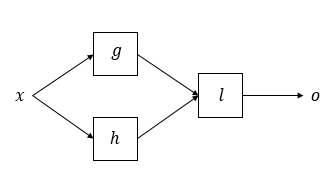
\includegraphics[width=0.4\linewidth]{graph2.png}
\end{figure}
\begin{itemize}
\item Simple example: input $x$, output $o$, various intermediate functions.
\item Chain rule gives us a way to compute gradient of $o$ with respect to $x$ by going \textit{backward} through intermediate nodes:
\begin{itemize}
\item Note $do/dl = 1$. 
\item First, find $\partial l / \partial g$ and $\partial l / \partial h$. 
\item Get gradients  $d g / d x$ and $d h / d x$.
\item Aggregate at $x$:
\begin{equation*}
\frac{d o}{dx} = \frac{\partial l}{\partial g} \frac{d g}{d x} + \frac{\partial l}{\partial h} \frac{dh}{dx}
\end{equation*} 
\end{itemize}
\end{itemize}

\end{frame}

\begin{frame}{Automatic Differentiation}

\begin{itemize}
\item Given a computation graph $f : x \to y$, we can automatically generate a new computation graph that returns $dy/dx$
\item (Very) roughly, each op in the graph is replaced by a gradients op that runs in the reverse-direction. Instead of the original op
%
\begin{equation*}
\mathcal{O} : x_1, ..., x_n \to y,
\end{equation*}
%
we place
%
\begin{equation*}
\mathcal{O}' : \frac{\partial *}{\partial y} \to \frac{\partial *}{\partial x_1}, ..., \frac{\partial *}{\partial x_n}
\end{equation*}
\item This procedure allows us to get gradients of any scalar signal (e.g. loss function) with respect to any inputs to a graph (e.g. trainable parameters)!
\end{itemize}
\end{frame}

\begin{frame}{Automatic Differentiation}
\begin{itemize}
\item You will almost never have to worry about what happens under the hood here
\item Libraries like Tensorflow, Theano, PyTorch, Caffe, and others take care of this for you
\item Takeaway: computation graph libraries let you define really complicated graphs (especially neural net architectures), get gradients for no extra programming effort, and easily optimize via first-order methods!
\end{itemize}
\end{frame}


\section{Tensorflow Basics}

\begin{frame}[fragile]{Basic Graph Building}

\begin{itemize}
\item Create points of data entry through \verb|tf.placeholder()|
\item Create parameter variables through \verb|tf.Variable()| or \verb|tf.get_variable()|\footnote{See https://stackoverflow.com/questions/37098546/difference-between-variable-and-get-variable-in-tensorflow}
\item Apply \textbf{operations} to data
\begin{itemize}
\item Can be simple/atomic
\begin{itemize}
\item In some places numpy syntax is supported (including broadcasting)
\item e.g. \verb|a + b| and \verb|tf.add(a,b)| produce same output
\end{itemize}
\item Or composite: see \verb|tf.layers| package for neural network layers
\begin{itemize}
\item e.g. \verb|tf.layers.dense()|, which creates standard feedforward `densely connected' neural net layer
\item Great for fast prototyping---most of the work already done for you! Snap pieces together like Lego
\end{itemize}
\end{itemize}
\end{itemize}

\end{frame}

\begin{frame}[fragile]{Example Graph Building}

From MNIST tutorial:

\begin{lstlisting}[language=python]
  # Create the model
  x = tf.placeholder(
        dtype=tf.float32, 
        shape=[None, 784]
        )
  W = tf.Variable(tf.zeros([784, 10]))
  b = tf.Variable(tf.zeros([10]))
  y = tf.matmul(x, W) + b
\end{lstlisting}

\end{frame}

\begin{frame}[fragile]{Operations Do Not Run At Define Time}

Caution!  Operations produce \textit{tensors} as outputs, not data.

\begin{lstlisting}[language=python]
In [3]: np.add(5,5)
Out[3]: 10

In [4]: tf.add(5,5)
Out[4]: <tf.Tensor 'Add:0' shape=() dtype=int32>
\end{lstlisting}

\end{frame}

\begin{frame}[fragile]{Session, Run, and Initialization}

\begin{itemize}
\item To compute outputs of CGs in TF, you need a Session. Several ways to get one:
\begin{itemize}
\item \verb|tf.Session()| 
\item \verb|tf.InteractiveSession()| (automatically sets as default)
\item \verb|tf.get_default_session()| (only if a default session exists)
\end{itemize}
\item Use the \verb|run()| command from a session to perform computations
\item \verb|run()| requires a \textbf{feed dict} for placeholders

\begin{lstlisting}[language=python]
sess = tf.InteractiveSession()
x_ph = tf.placeholder(shape=(None,100) ,dtype=tf.float32)
y_ph = tf.placeholder(shape=(None,10), dtype=tf.float32)
loss, update_op = build_network(x_ph, y_ph)
x_batch, y_batch = data_gen.next()
out = sess.run(
        [loss, update_op], 
        feed_dict={x_ph: x_batch, y_ph: y_batch}
        )
\end{lstlisting}
\end{itemize}

\end{frame}

\begin{frame}[fragile]{Further Notes on Run}

\begin{itemize}
\item \verb|run()| will only compute necessary pieces of computation graph to get outputs you ask for (nice---avoids excess compute!)
\item As on previous slide, \verb|run()| can get multiple outputs at once (with a single pass through necessary nodes in computation graph)
\item If you have variables in your computation graph, nothing will work until you initialize them
\begin{itemize}
\item To do this easily, after making session and graph, but before training:
\begin{lstlisting}[language=python]
sess.run(tf.global_variables_initializer())
\end{lstlisting}
\end{itemize}
\end{itemize}

\end{frame}

\begin{frame}[fragile]{Syntactic Sugar for Run}

\begin{itemize}
\item If just running one op / evaluating one Tensor, \textbf{and a default Session exists}, you can use \verb|.run()| and \verb|.eval()|\footnote{See https://stackoverflow.com/questions/38987466/eval-and-run-in-tensorflow}

\item \verb|.run()| works for \textbf{operations}
\begin{lstlisting}[language=python]
sess = tf.Session()
with sess.as_default():
  tf.global_variables_initializer().run()
\end{lstlisting}

\item \verb|.eval()| works for \textbf{tensors}
\begin{lstlisting}[language=python]
sess = tf.InteractiveSession()
x, y = make_inputs()
accuracy = build_network(x, y)
x_batch, y_batch = data_gen.next()
print(accuracy.eval(feed_dict={x : x_batch, y : y_batch}))
\end{lstlisting}
(In above snippet, recall that \verb|InteractiveSession| becomes default automatically!)

\end{itemize}

\end{frame}

\begin{frame}[fragile]{Loss Functions}

\begin{itemize}
\item Tensorflow makes common loss functions easy! Example, cross-entropy loss for classification:
\begin{lstlisting}[language=python]
# Create the model
x = tf.placeholder(tf.float32, [None, 784])
y = build_logits_network(x)

# Define loss and optimizer
y_ = tf.placeholder(tf.float32, [None, 10])

cross_entropy = tf.reduce_mean(
  tf.nn.softmax_cross_entropy_with_logits_v2(
    labels=y_, 
    logits=y
    )
  )
\end{lstlisting}
\item See \verb|tf.losses| for more (\verb|huber_loss|, \verb|hinge_loss|, etc.)
\item Watch out for \verb|softmax_cross_entropy| vs \verb|sparse_softmax_cross_entropy|
\end{itemize}
\end{frame}

\begin{frame}[fragile]{Loss Functions}
\begin{itemize}
\item Write your own custom losses. For instance, in policy gradients:
\begin{lstlisting}[language=python]
lr = tf.exp( logli - logli_old )
adv = tf.placeholder(shape=(None,), dtype=tf.float32)
surrogate_loss = -tf.reduce_mean( lr * adv )
\end{lstlisting}

\end{itemize}

\end{frame}

\begin{frame}[fragile]{Optimizers}

\begin{itemize}
\item After building networks and loss functions, \textbf{add an optimizer} to minimize loss.
\item Make an optimzer object, and set hyperparameters via constructor method (like momentum, RMSprop coefficients, Adam coefficients) or leave at safe defaults
\item Call minimize on loss to get training op:
\begin{lstlisting}[language=python]
optimizer = tf.train.AdamOptimizer(learning_rate=1e-3)
train_op = optimizer.minimize(loss)
\end{lstlisting}
\item To perform one step of training, just run training op!
\begin{lstlisting}[language=python]
sess.run(train_op, feed_dict)
\end{lstlisting}
\item NB: If you want to, you can specify which variables the optimizer acts on as an argument to \verb|minimize|
\end{itemize}

\end{frame}

\begin{frame}[fragile]{MNIST Example}

\lstset{style=mystyle2}

\begin{lstlisting}[language=python]
def main(_):
  # Import data
  mnist = input_data.read_data_sets(FLAGS.data_dir, one_hot=True)

  # Create the model
  x = tf.placeholder(tf.float32, [None, 784])
  W = tf.Variable(tf.zeros([784, 10]))
  b = tf.Variable(tf.zeros([10]))
  y = tf.matmul(x, W) + b

  # Define loss and optimizer
  y_ = tf.placeholder(tf.float32, [None, 10])

  cross_entropy = tf.reduce_mean(
    tf.nn.softmax_cross_entropy_with_logits(labels=y_, logits=y)
    )
  train_step = tf.train.GradientDescentOptimizer(0.5).minimize(cross_entropy)

  sess = tf.InteractiveSession()
  tf.global_variables_initializer().run()
  # Train
  for _ in range(1000):
    batch_xs, batch_ys = mnist.train.next_batch(100)
    sess.run(train_step, feed_dict={x: batch_xs, y_: batch_ys})

  # Test trained model
  correct_prediction = tf.equal(tf.argmax(y, 1), tf.argmax(y_, 1))
  accuracy = tf.reduce_mean(tf.cast(correct_prediction, tf.float32))
  print(sess.run(
              accuracy, 
              feed_dict={x: mnist.test.images, y_: mnist.test.labels}
              ))
\end{lstlisting}

\lstset{style=mystyle}

\end{frame}

\section{Building Advanced Computation Graphs}

\begin{frame}[fragile]{Common Neural Network Operations}

\begin{itemize}
\item Many standard neural network layers are already implemented, and enable high customization (for instance, custom initializers)
\item Dense / Fully-Connected layers ($Wx + b$):
\begin{itemize}
\item \verb|tf.layers.dense|
\item \verb|tf.contrib.layers.fully_connected|
\end{itemize}
\item Conv layers
\begin{itemize}
\item \verb|tf.layers.conv2d|
\item \verb|tf.contrib.layers.conv2d|
\end{itemize}
\item Activation functions: \verb|tf.nn.{relu, sigmoid, tanh, elu}|
\item Neural Network tricks: \verb|tf.layers.batch_normalization|, \verb|tf.layers.dropout|
\item Tensor utilities: \verb|tf.reshape|, \verb|tf.contrib.layers.flatten|, \verb|tf.concat|, \verb|tf.reduce_sum|, \verb|tf.reduce_mean|
\end{itemize}

\end{frame}

\begin{frame}[fragile]{Recurrent Neural Networks}

\begin{itemize}
\item To build a recurrent neural network (RNN), first specify an \textbf{RNN Cell}, which defines the computation at each time step. Note, this is \textit{not} the output Tensor you will run!
\begin{itemize}
\item \verb|tf.nn.rnn_cell.BasicRNNCell| ($h_t = \sigma(Wx_t + Rh_{t-1}+ b)$)
\item \verb|tf.nn.rnn_cell.GRUCell|
\item \verb|tf.nn.rnn_cell.LSTMCell|
\end{itemize}
\item Get a sequence of outputs and the final hidden state of an RNN computed with that Cell by calling \verb|tf.nn.dynamic_rnn|

\lstset{style=mystyle2}
\begin{lstlisting}[language=python]
In [1]: import tensorflow as tf
In [2]: x = tf.placeholder(shape=(None,None,10),dtype=tf.float32)
In [3]: cell = tf.nn.rnn_cell.GRUCell(20)
In [4]: outputs, final = tf.nn.dynamic_rnn(cell, x, time_major=False, dtype=tf.float32)
In [5]: sess = tf.InteractiveSession()
In [6]: tf.global_variables_initializer().run()
In [7]: import numpy as np
In [8]: o, f = sess.run([outputs, final], {x: np.random.rand(32,50,10)})
In [9]: o.shape
Out[9]: (32, 50, 20)
In [10]: f.shape
Out[10]: (32, 20)

\end{lstlisting}
\lstset{style=mystyle}

\end{itemize}

\end{frame}

\begin{frame}[fragile]{Variable Scoping and Reuse}

\begin{itemize}
\item Organize variables by name with variable scopes
\begin{lstlisting}[language=python]
out = input

with tf.variable_scope('conv1'):
    out = tf.layers.batch_normalization(out,...)
    out = tf.conv2d(out,...)

with tf.variable_scope('conv2'):
    out = tf.layers.batch_normalization(out,...)
    out = tf.conv2d(out,...)

\end{lstlisting}
\item Scopes can nest
\item Scope names become part of directory structure for variable names
\item Proper scoping helps when debugging
\end{itemize}
\end{frame}

\begin{frame}[fragile]{Variable Scoping and Reuse}
\begin{itemize}
\item Can reuse variables (ie make two nodes with tied weights) via reuse
\lstset{style=mystyle2}
\begin{lstlisting}[language=python]
In [1]: import tensorflow as tf
In [2]: x = tf.placeholder(shape=(None,10),dtype=tf.float32)
   ...: y = tf.placeholder(shape=(None,10),dtype=tf.float32)
   ...: with tf.variable_scope('test'):
   ...:     o1 = tf.layers.dense(x, 10)
   ...: with tf.variable_scope('test',reuse=True):
   ...:     o2 = tf.layers.dense(x, 10)
   ...:     
In [3]: o2
Out[3]: <tf.Tensor 'test_1/dense/BiasAdd:0' shape=(?, 10) dtype=float32>
In [4]: o1
Out[4]: <tf.Tensor 'test/dense/BiasAdd:0' shape=(?, 10) dtype=float32>
In [5]: tf.global_variables()
Out[5]: 
[<tf.Variable 'test/dense/kernel:0' shape=(10, 10) dtype=float32_ref>,
 <tf.Variable 'test/dense/bias:0' shape=(10,) dtype=float32_ref>]
\end{lstlisting}
\lstset{style=mystyle}
\item o1 and o2 are different tensors, but there is only one set of variables!
\item With \verb|reuse=tf.AUTO_REUSE|, variable name will determine reuse
\item Unintended variable reuse is a common source of bugs
\end{itemize}
\end{frame}


\begin{frame}[fragile]{Gradients and Stop Gradients}

\begin{itemize}
\item If you want to write a custom optimizer you may want to work with gradients directly; can do this using \verb|tf.gradients|
\item You may want to prevent backpropagation through a particular tensor: can do this with \verb|tf.stop_gradient|
\begin{itemize}
\item Example: in DQN, where we want to minimize a mean-square Bellman error with respect to params of current network but \textbf{not} target network

\lstset{style=mystyle3}
\begin{lstlisting}[language=python]
o = tf.placeholder(shape=(None,dim_o),dtype=tf.float32)
a = tf.placeholder(shape=(None,),dtype=tf.int32)
o2 = tf.placeholder(shape=(None,dim_o),dtype=tf.float32)
r = tf.placeholder(shape=(None,),dtype=tf.float32)
with tf.variable_scope('main'):
    q = build_network(o)                            # b x a
with tf.variable_scope('target'):
    q_targ = build_network(o2)                      # b x a
q_a = tf.reduce_sum(q * tf.one_hot(a, num_actions),1)   # b
q_targ_a = tf.reduce_max(q_targ,1)                      # b
target = r + gamma * q_targ_a
target = tf.stop_gradient(target)
loss = tf.reduce_mean(tf.square(q_a - target))
# later on, make assign statement so q_targ lags q 
\end{lstlisting}
\lstset{style=mystyle}

\end{itemize}
\end{itemize}

\end{frame}


\section{Logging and Debugging}

\begin{frame}[fragile]{Logging}

\begin{itemize}
\item Tensorflow has native operations for saving data through \verb|tf.summary|
\item Declare summary ops as functions of other tensors or ops\footnote{Example from \url{https://www.tensorflow.org/get_started/summaries_and_tensorboard}}
\lstset{style=mystyle2}
\begin{lstlisting}[language=python]
def variable_summaries(var):
  """Attach a lot of summaries to a Tensor (for TensorBoard visualization)."""
  with tf.name_scope('summaries'):
    mean = tf.reduce_mean(var)
    tf.summary.scalar('mean', mean)
    with tf.name_scope('stddev'):
      stddev = tf.sqrt(tf.reduce_mean(tf.square(var - mean)))
    tf.summary.scalar('stddev', stddev)
    tf.summary.scalar('max', tf.reduce_max(var))
    tf.summary.scalar('min', tf.reduce_min(var))
    tf.summary.histogram('histogram', var)

\end{lstlisting}
\lstset{style=mystyle}
\item Summary ops are never called unless you run them
\item For convenience, merge all summary ops via
\begin{lstlisting}[language=python]
merged_summary_op = tf.summary.merge_all()
\end{lstlisting}

\end{itemize}
\end{frame}

\begin{frame}[fragile]{Logging}

\begin{itemize}
\item Make a \verb|tf.summary.FileWriter| to save summaries to file.\footnote{\url{https://www.tensorflow.org/api_docs/python/tf/summary/FileWriter}}
\lstset{style=mystyle3}
\begin{lstlisting}[language=python]
...create a graph...
# Launch the graph in a session.
sess = tf.Session()
# Create a summary writer, add the 'graph' to the event file.
writer = tf.summary.FileWriter(<some-directory>, sess.graph)
\end{lstlisting}
\lstset{style=mystyle}
Passing the graph into FileWriter allows you to inspect the computation graph later when you visualize in TensorBoard.
\item To save summaries with the FileWriter, run the merged summary op and then use \verb|add_summary|:
\lstset{style=mystyle3}
\begin{lstlisting}[language=python]
for i in range(n_steps):
  feed_dict = get_next_feed_dict()
  summary, _ = sess.run([merged_summary_op, train_op], feed_dict)
  writer.add_summary(summary, i)
\end{lstlisting}
\end{itemize}

\end{frame}

\begin{frame}[fragile]{Logging}

\begin{figure}
  \centering
  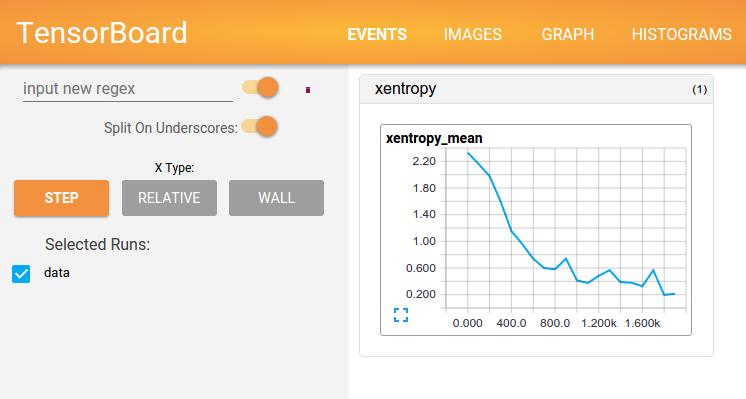
\includegraphics[width=0.8\linewidth]{mnist_tensorboard.png}
\end{figure}

Invoke Tensorboard with \verb|tensorboard --logdir=path/to/log-directory|

\end{frame}

\begin{frame}[fragile]{Debugging}

\begin{itemize}
\item Explore with \verb|InteractiveSession| in IPython
\item Common issue---Tensor shapes are wrong. Can check with \verb|<tensor>.get_shape().as_list()|.
\item Want to look at the list of all variables? \verb|tf.global_variables()|.

\lstset{style=mystyle2}
\begin{lstlisting}[language=python]
In [1]: import tensorflow as tf

In [2]: x = tf.placeholder(shape=(None,10), dtype=tf.float32)

In [3]: with tf.variable_scope('test'):
   ...:     y = tf.layers.dense(x, 20)
   ...:     

In [4]: tf.global_variables()
Out[4]: 
[<tf.Variable 'test/dense/kernel:0' shape=(10, 20) dtype=float32_ref>,
 <tf.Variable 'test/dense/bias:0' shape=(20,) dtype=float32_ref>]
\end{lstlisting}
\item Good scoping makes it easier to find problem areas
\item Inject print ops into your graph (see \verb|tf.Print|, \verb|tf.print|)
\end{itemize}


\end{frame}

\begin{frame}{Debugging}
\begin{itemize}
\item Sometimes, look at raw inputs and outputs of networks!
\begin{itemize}
\item If outputs all look the same despite different inputs, maybe a hidden layer's activations are saturating
\end{itemize}
\item Be \textit{super} careful about BatchNorm and other neural network tricks that have different behavior at training time and test time
\begin{itemize}
\item See reference\footnote{http://ruishu.io/2016/12/27/batchnorm/} for a good guide on using BatchNorm correctly.
\end{itemize}
\item Make sure the scale of inputs to your network is reasonable (empirically it helps sometimes for data to have mean zero and std=1)
\item If you are using default values anywhere (in layers, optimizers, etc.), \textbf{check them} and make sure they make sense
\end{itemize}
\end{frame}


\section{What Else is Out There?}

\begin{frame}{Computation Graph Libraries}

\begin{itemize}
\item Tensorflow (Google) - Huge community, well-supported, somewhat clunky API but great distributed performance
\item Theano (U of Montreal) - Long history, widely-used, slow to compile
\item Caffe (Berkeley / Facebook)
\item Torch (Facebook and others) - Now available in Python (previously just Lua), define-by-run makes for fast and flexible prototyping, comparable speed to Tensorflow
\item Chainer (Preferred Networks) - Another define-by-run like Torch
\end{itemize}

For some performance comparisons:
\url{https://github.com/soumith/convnet-benchmarks}


\end{frame}

\begin{frame}{Additional APIs/Wrappers for Tensorflow}

\begin{itemize}
\item tf-contrib (active development code in Tensorflow available to user, usually stabilizes into main code eventually)
\item Keras (officially supported by Google)
\item Sonnet (supported by Deepmind! which is owned by Go---wait a second... how many APIs did Google make for this thing?)
\item TFLearn
\end{itemize}

Lots of fragmentation, but things seem to have stabilized around core Tensorflow / Keras. Sonnet may be worth watching, though, because of DeepMind. 

\end{frame}

\begin{frame}{That's All Folks}

Questions?

\end{frame}

\end{document}